
\noindent \textbf{L4.2 (Sipser 2.9)} Dê uma gramatica livre-do-contexto que gere a linguagem
\begin{center}
$A = \{a^ib^jc^k \ |\ i = j$ ou $j = k$ onde $i, j, k \geq 0\}$
\end{center}

\textbf{Resposta: } A GLC que gera a linguagem $A$ é $G = (\{S, S_1, S_2, A, C\}, \{a, b, c\}, R, S)$, onde $S$ é a variável inicial e $R$ é o conjunto de regras:
\begin{align*}
    S &\rightarrow AS_2 \ |\ S_1C \\
    S_1 &\rightarrow aS_1b \ |\ \epsilon \\
    S_2 &\rightarrow bS_2c \ |\ \epsilon \\
    A &\rightarrow aA \ |\ \epsilon \\
    C &\rightarrow cC \ |\ \epsilon \\
\end{align*}

\textbf{Sua gramática é ambígua? Por que ou por que não?}\\[3pt]
Sim, ela é ambígua, pois $G$ gera uma mesma cadeia, digamos $w$, ambiguamente, ou seja, $w$ tem duas árvores sintáticas distintas. A derivação da cadeia $w = abc$, por exemplo, produz duas árvores sintáticas diferentes.

\begin{figure}[H]
\begin{tikzpicture}[sibling distance=72pt]
\Tree [.$S$ [.$S_1C$ [.$aS_1b$ $ab$ ] [.$cC$ $c$ ] ] ]
\end{tikzpicture}
%
\begin{tikzpicture}[sibling distance=72pt]
\Tree [.$S$ [.$AS_2$ [.$aA$ $a$ ] [.$bS_2c$ $bc$ ] ] ]
\end{tikzpicture}
\centering
\end{figure}
